\documentclass[border=3mm]{standalone}
\usepackage{tikz}
\usetikzlibrary{intersections}
\usetikzlibrary{angles,quotes}% angles
\usetikzlibrary{arrows}% arrows
\tikzset{>=latex}
\newenvironment{standalonepage}{}{}%keep pictures on same page
\standaloneenv{standalonepage}

% START basic figure
% no empty line between \tikzset and myfige/.pic={
\tikzset{% 
  myfig/.pic={%
    \begin{scope}[scale=4]% must match scale in tikzpicture below
      
      % set up basic coordinates
      \coordinate (A) at (-1,+1); 
      \coordinate (B) at (+1,+1);
      \coordinate (C) at (+1,-1);
      \coordinate (D) at (-1,-1);
      
      % draw square with labels
      \draw (A) node[above left] {$A$} -- node[midway, above] {$1$} (B) node[above right] {$B$} -- (C) node[below right] {$C$} -- (D) node[below left] {$D$} -- cycle;
    
      % find the intersection between BC and 20-degree angle at A
      \path [name path=AF] (A) -- +(-20:2.3cm);
      \path [name path=BC] (B) -- (C);
      \path [name intersections={of=AF and BC, by=F}];
      \node [right] at (F) {$F$};
      
      % find the intersection between DC and 65-degree angle at A
      \path [name path=AE] (A) -- +(-65:2.3cm);
      \path [name path=DC] (D) -- (C);
      \path [name intersections={of=AE and DC, by=E}];
      \node [below] at (E) {$E$};
    
    \end{scope}
  }%
}%
% END basic figure


\begin{document}


\begin{standalonepage}
  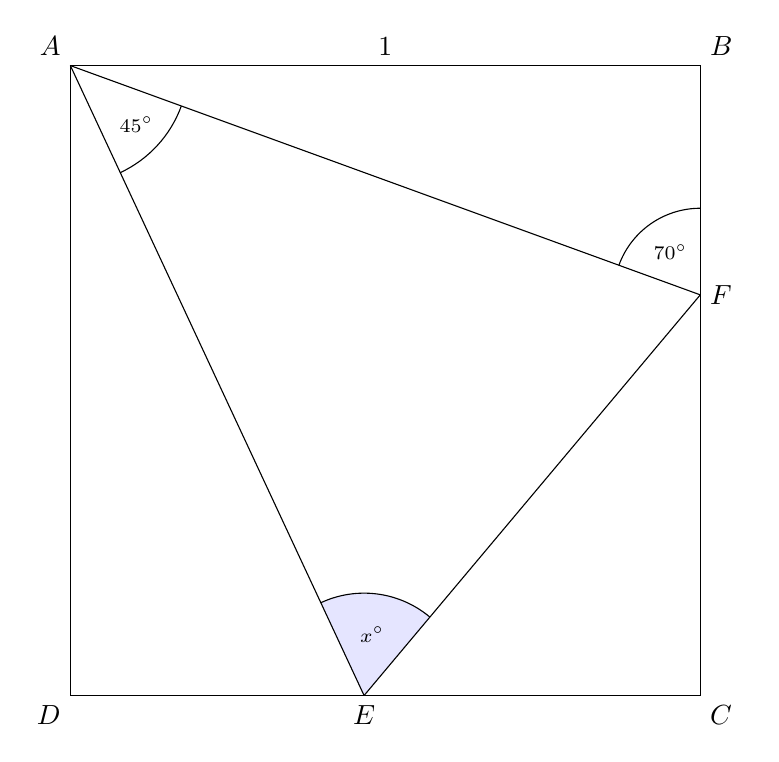
\begin{tikzpicture}
  
    \pic {myfig};
    
    % NOTE: was unable to include the next few commands inside \tikzset
    % So including it here, and copy-pasting again below
  
    % mark the angle at EAF
    \pic [draw=black, text=black, font=\scriptsize, angle radius=1.5cm, "$45^{\circ}$"{xshift=5pt,yshift=-4pt}]{angle=E--A--F};
  
    % mark the angle at BFA
    \pic [draw=black, text=black, font=\scriptsize, angle radius=1.1cm, "$70^{\circ}$"]{angle=B--F--A};
    
    % mark the unknown angle at FEA
    \pic [fill=blue!10, draw=black, text=black, font=\scriptsize, angle radius=1.3cm, "$x^{\circ}$"]{angle=F--E--A};
  
    % draw the AE, AF, EF lines last
    \draw (A) -- (F);
    \draw (A) -- (E);
    \draw (E) -- (F);
    
  \end{tikzpicture}
\end{standalonepage}


\begin{standalonepage}
  \begin{tikzpicture}[scale=4]% must match scope in myfig
  
    \pic (original) {myfig};
  
    % mark the angle at EAF
    \pic [draw=black, text=black, font=\scriptsize, angle radius=1.5cm, "$45^{\circ}$"{xshift=5pt,yshift=-4pt}]{angle=E--A--F};
  
    % mark the angle at BFA
    \pic [draw=black, text=black, font=\scriptsize, angle radius=1.1cm, "$70^{\circ}$"]{angle=B--F--A};
  
    % mark the angle at FAB
    \pic [draw=red, text=red, font=\scriptsize, angle radius=1.5cm, "$20^{\circ}$"{xshift=7pt,yshift=0pt}]{angle=F--A--B};
    
    % mark the right angle at ABF
    \begin{scope}[rotate=90]
    \draw [red] (B) +(-2mm,0) |- +(0,2mm) node[shift={(11pt,-11pt)}, text=red, font=\scriptsize] {$90^{\circ}$};
    \end{scope}
      
    % draw the AE, AF, EF lines last
    \draw (A) -- (F);
    \draw (A) -- (E);
    \draw (E) -- (F);
    
  \end{tikzpicture}
\end{standalonepage}



\begin{standalonepage}
  \begin{tikzpicture}[scale=4]% must match scope in myfig
  
    \pic (original) {myfig};
  
    % mark the angle at EAF
    \pic [draw=black, text=black, font=\scriptsize, angle radius=1.5cm, "$45^{\circ}$"{xshift=5pt,yshift=-4pt}]{angle=E--A--F};
  
    % mark the angle at BFA
    \pic [draw=black, text=black, font=\scriptsize, angle radius=1.1cm, "$70^{\circ}$"]{angle=B--F--A};
  
    % mark the angle at FAB
    \pic [draw=black, text=black, font=\scriptsize, angle radius=1.5cm, "$20^{\circ}$"{xshift=7pt,yshift=0pt}]{angle=F--A--B};
  
    % mark the angle at DAE
    \pic [draw=red, text=red, font=\scriptsize, angle radius=1.5cm, "~$25^{\circ}$"{xshift=1.5pt,yshift=-8pt}]{angle=D--A--E};
    
    % mark the right angle at ADE
    \begin{scope}[rotate=-90]
    \draw [red] (D) +(-2mm,0) |- +(0,2mm) node[shift={(-10pt,10pt)}, text=red, font=\scriptsize] {$90^{\circ}$};
    \end{scope}
  
    % mark the angle at AED
    \pic [draw=red, text=red, font=\scriptsize, angle radius=1.1cm, "~$65^{\circ}$"]{angle=A--E--D};
  
    % draw the AE, AF, EF lines last
    \draw (A) -- (F);
    \draw (A) -- (E);
    \draw (E) -- (F);
    
  \end{tikzpicture}
\end{standalonepage}


\begin{standalonepage}
  \begin{tikzpicture}[scale=4]% must match scope in myfig
  
    \pic (original) {myfig};
  
    % mark the angle at EAF
    \pic [draw=black, text=black, font=\scriptsize, angle radius=1.5cm, "$45^{\circ}$"{xshift=5pt,yshift=-4pt}]{angle=E--A--F};
  
    % mark the angle at BFA
    \pic [draw=black, text=black, font=\scriptsize, angle radius=1.1cm, "$70^{\circ}$"]{angle=B--F--A};
  
    % mark the angle at FAB
    \pic [draw=black, text=black, font=\scriptsize, angle radius=1.5cm, "$20^{\circ}$"{xshift=7pt,yshift=0pt}]{angle=F--A--B};
  
    % mark the angle at DAE
    \pic [draw=black, text=black, font=\scriptsize, angle radius=1.5cm, "~$25^{\circ}$"{xshift=1.5pt,yshift=-8pt}]{angle=D--A--E};
  
    % draw the AE, AF, EF lines last
    \draw (A) -- (F);
    \draw (A) -- (E);
    \draw (E) -- (F);
  
    % find the intersection between DC and 20-degree angle at A
    \path [name path=AG] (A) -- +(-110:2.2cm);
    \path [name path=CD] (C) -- +(-2.8,0);
    \path [name intersections={of=AG and CD, by=G}];
    \node [below] at (G) {$F^{\prime}$};
  
    % draw the AF' lines last
    \draw [red] (A) -- (G);
    \draw [red] (G) -- (D);
  
    % mark the angle at GAD
    \pic [draw=red, text=red, font=\scriptsize, angle radius=1.5cm, "$20^{\circ}$"{xshift=-1.5pt,yshift=-10pt}]{angle=G--A--D};
    
    % mark the right angle at ADG
    \begin{scope}[rotate=0]
    \draw [red] (D) +(-2mm,0) |- +(0,2mm) node[shift={(-10pt,-10pt)}, text=red, font=\scriptsize] {$90^{\circ}$};
    \end{scope}
  
    % mark the angle at DGA
    \pic [draw=red, text=red, font=\scriptsize, angle radius=1.1cm, "$70^{\circ}$"]{angle=D--G--A};
    
  \end{tikzpicture}
\end{standalonepage}



\begin{standalonepage}
  \begin{tikzpicture}[scale=4]% must match scope in myfig
  
    \pic (original) {myfig};
  
    % mark the angle at EAF
    \pic [draw=black, text=black, font=\scriptsize, angle radius=1.5cm, "$45^{\circ}$"{xshift=5pt,yshift=-4pt}]{angle=E--A--F};
  
    % mark the angle at BFA
    \pic [draw=black, text=black, font=\scriptsize, angle radius=1.1cm, "$70^{\circ}$"]{angle=B--F--A};
  
    % draw the AE, AF, EF lines last
    \draw (A) -- (F);
    \draw (A) -- (E);
    \draw (E) -- (F);
  
    % find the intersection between DC and 20-degree angle at A
    \path [name path=AG] (A) -- +(-110:2.2cm);
    \path [name path=CD] (C) -- +(-2.8,0);
    \path [name intersections={of=AG and CD, by=G}];
    \node [below] at (G) {$F^{\prime}$};
  
    % draw the AF' lines last
    \draw [red] (A) -- (G);
    \draw [red] (G) -- (D);
  
    % mark the angle at GAE
    \pic [draw=red, text=red, font=\scriptsize, angle radius=1.5cm, "$45^{\circ}$"{xshift=0.5pt,yshift=-5pt}]{angle=G--A--E};
  
    % mark the angle at DGA
    \pic [draw=red, text=red, font=\scriptsize, angle radius=1.1cm, "$70^{\circ}$"]{angle=D--G--A};
  
    % mark the angle at AFE
    \pic [draw=red, text=red, font=\scriptsize, angle radius=1.1cm, "$70^{\circ}$"]{angle=A--F--E};
    
    \draw [->,red,thick] (-1.5,-0.85) to[bend left] (0.73,0.2);
  
  \end{tikzpicture}
\end{standalonepage}



\begin{standalonepage}
  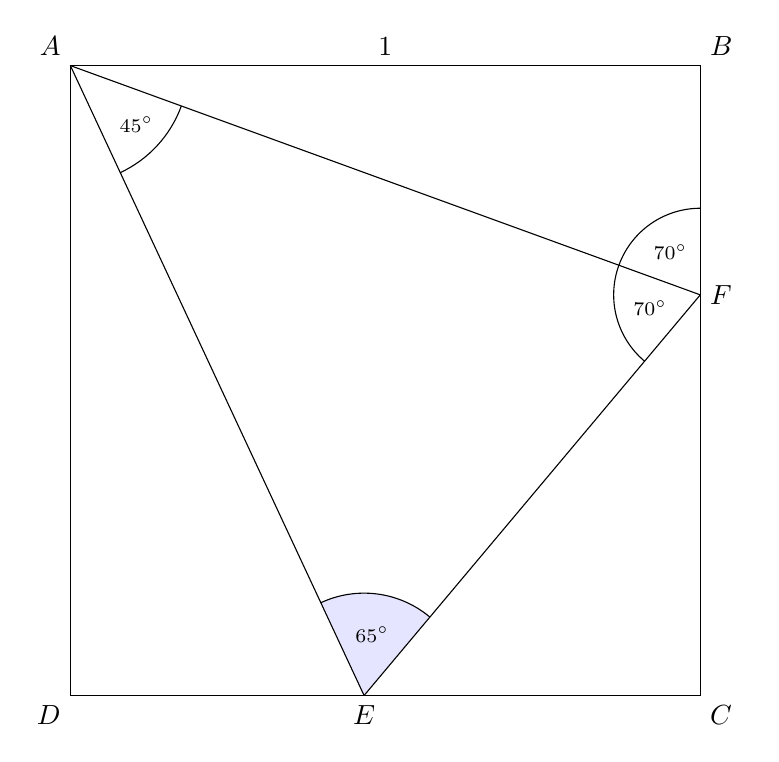
\begin{tikzpicture}
  
    \pic {myfig};
  
    % mark the angle at EAF
    \pic [draw=black, text=black, font=\scriptsize, angle radius=1.5cm, "$45^{\circ}$"{xshift=5pt,yshift=-4pt}]{angle=E--A--F};
  
    % mark the angle at BFA
    \pic [draw=black, text=black, font=\scriptsize, angle radius=1.1cm, "$70^{\circ}$"]{angle=B--F--A};
    
    % mark the unknown angle at FEA
    \pic [fill=blue!10, draw=black, text=black, font=\scriptsize, angle radius=1.3cm, "$65^{\circ}$"]{angle=F--E--A};
  
    % draw the AE, AF, EF lines last
    \draw (A) -- (F);
    \draw (A) -- (E);
    \draw (E) -- (F);
  
    % mark the angle at AFE
    \pic [draw=black, text=black, font=\scriptsize, angle radius=1.1cm, "$70^{\circ}$"]{angle=A--F--E};
    
  \end{tikzpicture}
\end{standalonepage}


\end{document}
